\chapter{识别PE模型性能对比及分析}
\section{引言}
此前的章节已经完成了机器学习任务的所需的数据的所有预处理,本章开始将使用真正的机器学习模型与相关算法开始分析工作。
本章主要介绍了本研究所涉及的机器学习的监督学习、无监督学习、集成学习及深度学习领域的部分算法及原理。出于篇幅的考虑,各领域均只选取了1-2种经典算法进行介绍。
所有算法的具体性能及分析等可参见下一章节的内容。

\section{基本机器学习模型的应用(监督学习)}
本小节对本研究涉及的机器学习中经典监督学习的算法模型进行介绍。

\subsection{决策树}
决策树(Decision Tree,DT)是数据挖掘的经典算法之一,是一种类似流程图的树结构,可以用于连续数值型变量的回归预测及离散型数值型变量的分类问题\cite{Li2017,Liu2018}。
决策树算法的最显著优点是简单直观,易于可视化、可读性强。

一、决策树的结构与原理

分类决策树模型是对实例进行分类的树形结构的描述,如\autoref{fig:dt}所示。一般而言,决策树由结点和有向边组成,而结点又可分为内部结点与叶节点。其中,前者表示一个特征或属性,后者对应决策结果,一般是一个类\cite{Li2017,Zhou2016}。
决策树可以看成一个if-else规则的集合,决策树的根节点到叶节点的每条路径分别对应着一条规则:路径上的内部结点集合构成了规则的判断条件,而叶节点所属的具体类则对应着该规则的结论。
决策树的学习目的就是从训练数据集中集中归纳出一组分类规则,产生一颗与训练数据的矛盾小的、泛化能力强的逻辑判断树。
\begin{figure}[htbp]
    \centering
    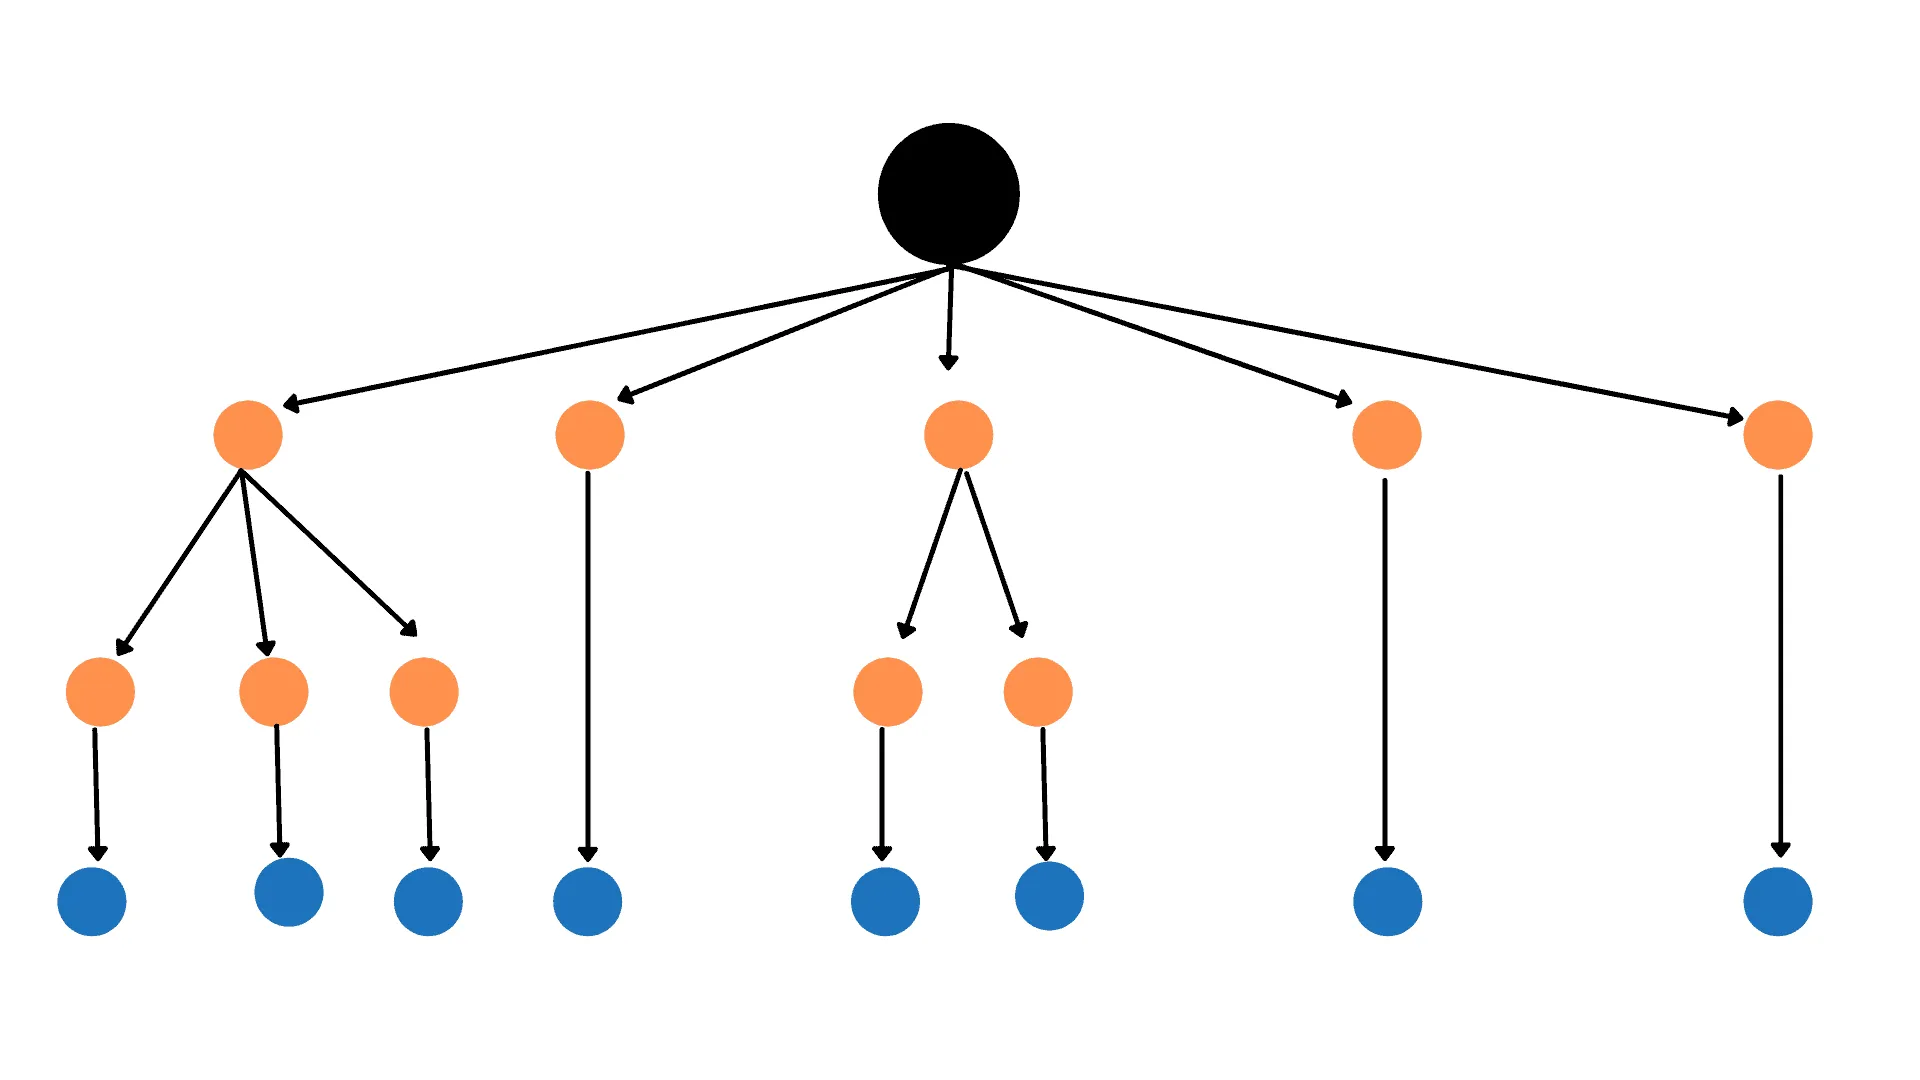
\includegraphics[width=.6\linewidth]{models/dt3.png}
    \caption{\label{fig:dt}决策树模型示意}
\end{figure}

二、决策树的构建

决策树的生成构建过程一般是一个递归地选择最优特征,并根据最优特征对训练数据进行分割,使该分割对各个新的子数据集有最优分类效果的过程。

\begin{breakablealgorithm}
    \caption[CART生成算法]{CART递归生成算法\cite{Li2017}}
    \label{alg:cart}
    \begin{algorithmic}[1] %每行显示行号
        \Require 训练数据集$D$。
        \Ensure CART决策树。
        \State 建立一颗空树$CART$,设该树的根结点为$root$。
        \Function{GenerateCart}{$CART,D_0,root$}
            \State $D_0$为当前结点的训练数据集,计算现有特征对该数据集的基尼指数。对每一个特征$A$,对其可能取的每个值$a$,根据样本点对$A=a$的测试为“是”或“否”将$D_0$分割成$D_l$与$D_r$两部分,计算$A=a$时的基尼指数。
            \State 在所有可能的特征$A$以及它们所有可能的切分点$a$中,选择基尼指数最小的特征及其对应的切分点作为最有特征与最优切分点。
            \State 依最优特征与最优切分点,从现结点生成两个子节点$left$与$right$,将训练数据集依特征分配到两个子节点中去,即$D_l$与$D_r$。更新当前$CART$。
            \If {结点中的样本个数小于预定阈值 \textbf{or} 样本集的基尼指数小于预定阈值 \textbf{or} 没有更多特征}
                \State \Return{$CART$}
            \Else    
                \State \Call{GenerateCart}{$CART,D_l,left$}
                \State \Call{GenerateCart}{$CART,D_r,right$}
            \EndIf
        \EndFunction
    \end{algorithmic}
\end{breakablealgorithm}


\subsection{常见的监督学习方法}

\section{基本机器学习模型的应用(无监督学习)}
\subsection{常见的无监督学习方法}
\subsection{Kmeans}
\begin{figure}[htbp]
    \centering
    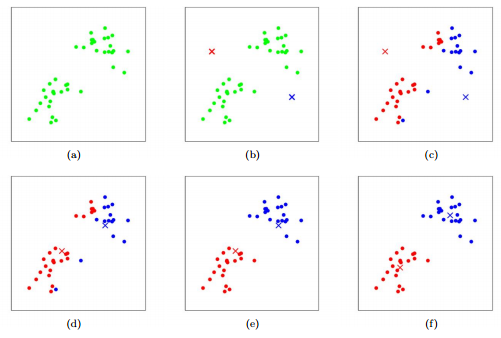
\includegraphics[width=.6\linewidth]{models/kmeans}
    \caption[Kmeans算法运行示意]{\label{fig:kmeans}Kmeans算法运行示意\cite{kmeans}。训练示例显示为点,簇质心显示为十字。(a) 原始数据集。(b) 随机初始簇质心。(c-f)运行两次k均值迭代的说明。在每次迭代中,我们将每个训练示例分配给最接近的聚类质心。}
\end{figure}


\begin{breakablealgorithm}
    \caption[KMeans聚类算法]{KMeans聚类算法\cite{Zhou2016}}
    \label{alg:kmean}
    \begin{algorithmic}[1] %每行显示行号
        \Require 样本集$D=\{x_1,x_2,\dots,x_m\}$,聚类簇数$k$。
        \Ensure 簇划分$C=\{C_1,C_2,\dots,C_k\}$
        \State 从D中随机选择k个样本作为初始均值向量$\{\mu_1,\mu_2,\dots,\mu_k\}$
        \Repeat
        \State 令$C_i=\emptyset (1\le i\le k)$
            \For {$j=1,2,\dots,m$}
                \State 计算样本$x_j$与各均值向量$\mu_i (1\le i \le k)$的距离:$d_{ij}={||x_j - \mu_j||}_2$
                \State 根据距离最近的均值向量确定$x_j$的簇标记:$\lambda_j = \arg \min_{i \in \{1,2,\dots,k\}} d_{ij}$
                \State 将样本$x_j$划入对应的簇:$C_{\lambda_j} = C_{\lambda_j} \cup \{x_j\}$
            \EndFor
            \For {$i=1,2,\dots,k$}
                \State 计算新均值向量:$\mu_i^{'}=\frac{1}{|C_i|} \sum_{x \in C_i}{x}$
                \If {$\mu_i^{'} \ne \mu_i$}
                    \State 将当前均值向量$\mu_i$更新为$\mu_i^{'}$
                \Else
                    \State 保持当前均值向量不变
                \EndIf
            \EndFor
        \Until 当前均值向量均未更新
    \end{algorithmic}
\end{breakablealgorithm}
\section{集成学习的应用}
\subsection{常见的集成学习方法}
\subsection{Adboost}
\subsection{随机森林}
随机森林

\section{深度学习模型的应用}
\section{小结}
